\begin{multicols}{2}

%Interpeting the PET/CT image

With the complementary strengths of PET and CT scanners assessing tumor margins and guiding surgical interventions is possible. In the case for staging and diagnosing PDAC, PET/CT achieves sensitivity rates of 89–91\% and specificity rates of 70–72\% in detecting PDAC lesions \cite{TG174}.

PET/CT is used in clinical settings in various applications. It excels at identifying primary tumors and detecting distant metastases by FDG concentrated regions lighting up. In a following example, Zhang et al. demonstrated its utility in detecting rare metastatic sites, such as cutaneous and muscle involvement\cite{Zhang2023}. Additionally, PET/CT is invaluable for evaluating lymph node involvement, as lymph nodes often act as early sites for metastasis. When FDG concentrates it shows increased glucose metabolism due to cancer activity. This is unique information from PET since lymph nodes may appear normal in size on CT but are metabolically active. Accurate identification of these cancerous nodes improves staging precision, which is critical for planning surgeries, such as lymphadenectomy (removal of affected nodes), and for deciding if curative treatments are feasible \cite{TG174}.  Furthermore, while FDG uptake is non-specific, combining PET/CT with clinical markers (e.g., IgG4 levels) can help  distinguish between similar conditions, such as autoimmune pancreatitis and pancreatic ductal adenocarcinoma. This is also better illustrated in a following case studie reported by Zheng, Et al. \cite{Zheng2018}.

Another one of the emerging technologies is the Total Body PET/CT systems. This devices seek to enable whole-body imaging in a single scan, hopefully with enhanced resolution and reduced scanning time \cite{SunderlandSeminar}.The main differences come from the increased FOV for whole body (>1m) which in return increases senstivity and enables whole-body dynamic imaging and parametric imaging, providing real-time insights into tracer distribution and kinetics across all organs simultaneously. This is a valuable innovation for early detecting micrometastases and monitoring therapeutic responses.

%\section{Applications of [18F]FDG-PET/CT}

PET/CT can be of great help during the different parts of treatment, from diagnosis, staging, to management of pancreatic cancer. In order to exemplify its applications three clinical cases are introduced:

\begin{itemize}
	\item \textbf{Case 1 - Zheng et al.:} 
	A 46-year-old male  with suspected pancreatic cancer presented, in 2018, a metabolic active lesion was suspected from a CT scan. This lesion is located in the tail of pancreas and had hinted overlap of metabolic signatures typical of both malignancy and autoimmune pancreatitis\cite{Zheng2018}.
	\item \textbf{Case 2 - Zhang et al.:} 
	In 2023 case, a 61-year-old male with confirmed pancreatic adenocarcinoma and treated with radical resection 6 years earlier presented rare metastatic sites and was reevaluated\cite{Zhang2023}.
	\item \textbf{Case 3 - Deng et al.:} 
	Study in 2021 that compared FDG with 68Ga-FAPI, Gallium-68-labeled Fibroblast Activation Protein Inhibitor, in a 65-year-old female with pancreatic cancer and liver metastases. DG-PET/CT identified hypermetabolic liver lesions, but 68Ga-FAPI demonstrated superior sensitivity in delineating hypodense metastases\cite{Deng2021}.
\end{itemize}

These cases together exemplify applications in the diagnosis and staging of pancreatic cancer of this imaging modality.


%---

% Case 1 Zheng
\subsection{Treatment Planning and Monitoring}

\textbf{Guiding Therapy with PET/CT:} In order to perform a surgical resection and radiation therapy the boundaries of the tumor must be carfully delinated. Zheng et al. were able to differentiate autoimmune pancreatitis from PDAC from this images, avoiding unnecessary or ineffective treatments \cite{Zheng2018}.

From case 1, figure \ref{fig:Zheng1} A) shows a maximum density projection (MIP) from a PET scanner that revealed several areas of increased FDG uptake, with SUV values of 8.4, indicating potential pancreatic cancer. Shown with the thick arrow. Additionally showed increased activity in the regions of the salivary glands (small arrows), in the region of  lymph nodes (arrowheads).

On axial image (B: PET, C: CT, D: fusion), the left upper abdominal activity (arrows) corresponded to an irregular, slightly low in density mass measuring about $8.2 \times 8.0 \times 8.1 \text{cm}$ in the pancreatic tail on the CT and fusion images. The PET/CT results were still suggestive of a pancreatic malignancy. However,
the increased activity in the salivary gland and  lymph nodes raised the possibility of type 1 autoimmune pancreatitis

Figure~\ref{fig:Zheng1} showcases how PET/CT identifies metabolic distinctions that inform treatment in challenging cases where inflammatory and malignant lesions overlap. Additionally, post-treatment PET/CT imaging provides insights into metabolic response, that enables clinicians to adjust therapeutic regimens based on observed changes in FDG uptake. 

\textbf{Enhancing Planning with Alternative Tracers:} As noted in Deng et al., the integration of new tracers like 68Ga-FAPI offers improved sensitivity in hypoxic tumor regions. \cite{Deng2021}.

\end{multicols}

\begin{figure}[ht]
	\centering
	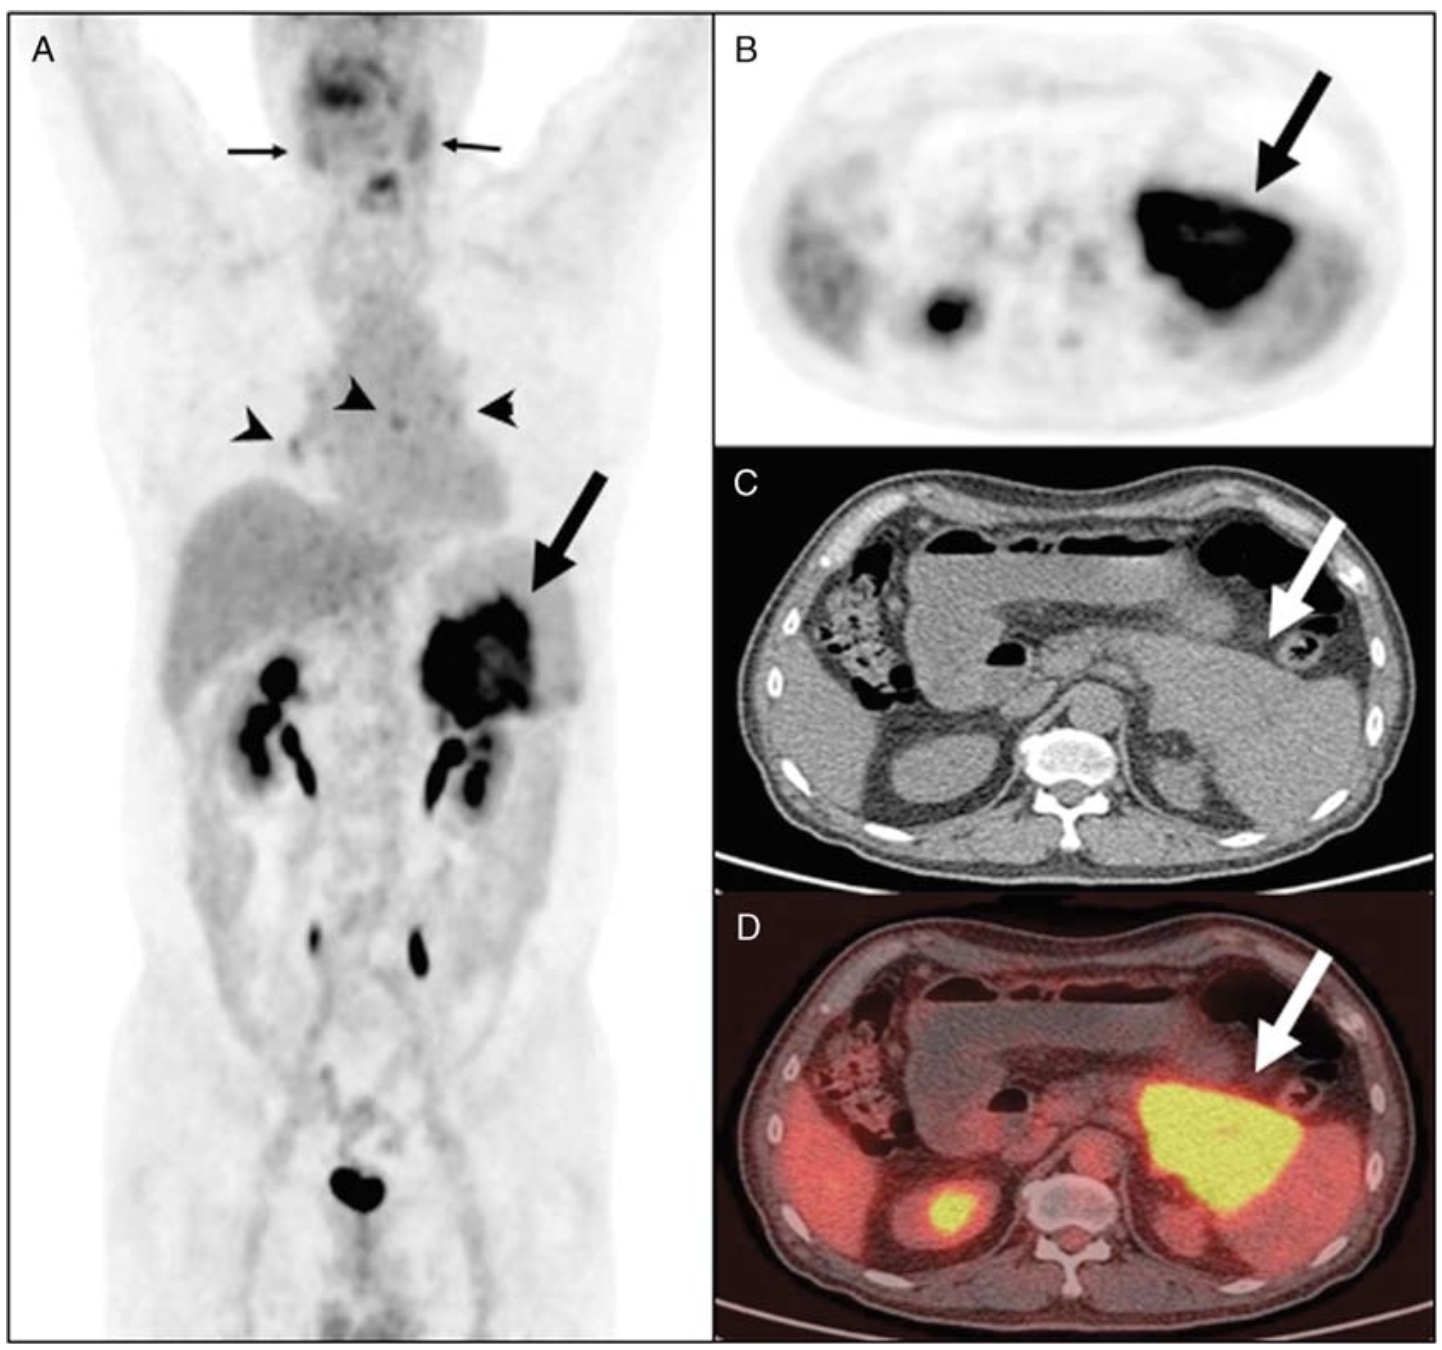
\includegraphics[width=0.65\textwidth]{assets/Zheng1.png}
	\caption{FDG-PET/CT imaging showing focal autoimmune pancreatitis mimicking pancreatic cancer. Note: the overlapping metabolic activity that challenges differentiation \cite{Zheng2018}.}
	\label{fig:Zheng1}
\end{figure}

%---

\begin{multicols}{2}


%Case 2 - Zhang
\subsection{Lymph Node Evaluation and Metastasis Detection}

\textbf{Unique Metastases:} 
In case 2, PET/CT demostrated its capacity to distiguish between muscle and cutaneous metastases from PDAC—locations rarely detected by conventional imaging. Without PET/CT this would be possible to asses correctly

Figure~\ref{fig:Zhang1}, depicts a MIP image with two regions of elevated glucose metabolism (Upper abdomen and left lateral abdominal wall). An axial image of the anatomy shows near the surgery site that shows elevated metabolic activity, possibly indicating residual or recurrent cancer, or post-surgical inflammatory changes. Then focused on the lateral it shows an hypodense structure seen in the muscle. This is the rare case of a metastatic deposit in the muscle. They highlight that muscle metastases from pancreatic cancer are exceptionally rare, while cutaneous metastases occur in only 0.5–7.6\% of cases, often at the umbilicus\cite{Zhang2023}.


\textbf{Sensitivity and Specificity:} Zhang et al. found that FDG uptake reliably identifies malignancies, it may also highlight non-malignant inflammatory processes, necessitating careful interpretation and, when possible, the inclusion of additional clinical markers or advanced tracers.


\end{multicols}

\begin{figure}[ht]
	\centering
	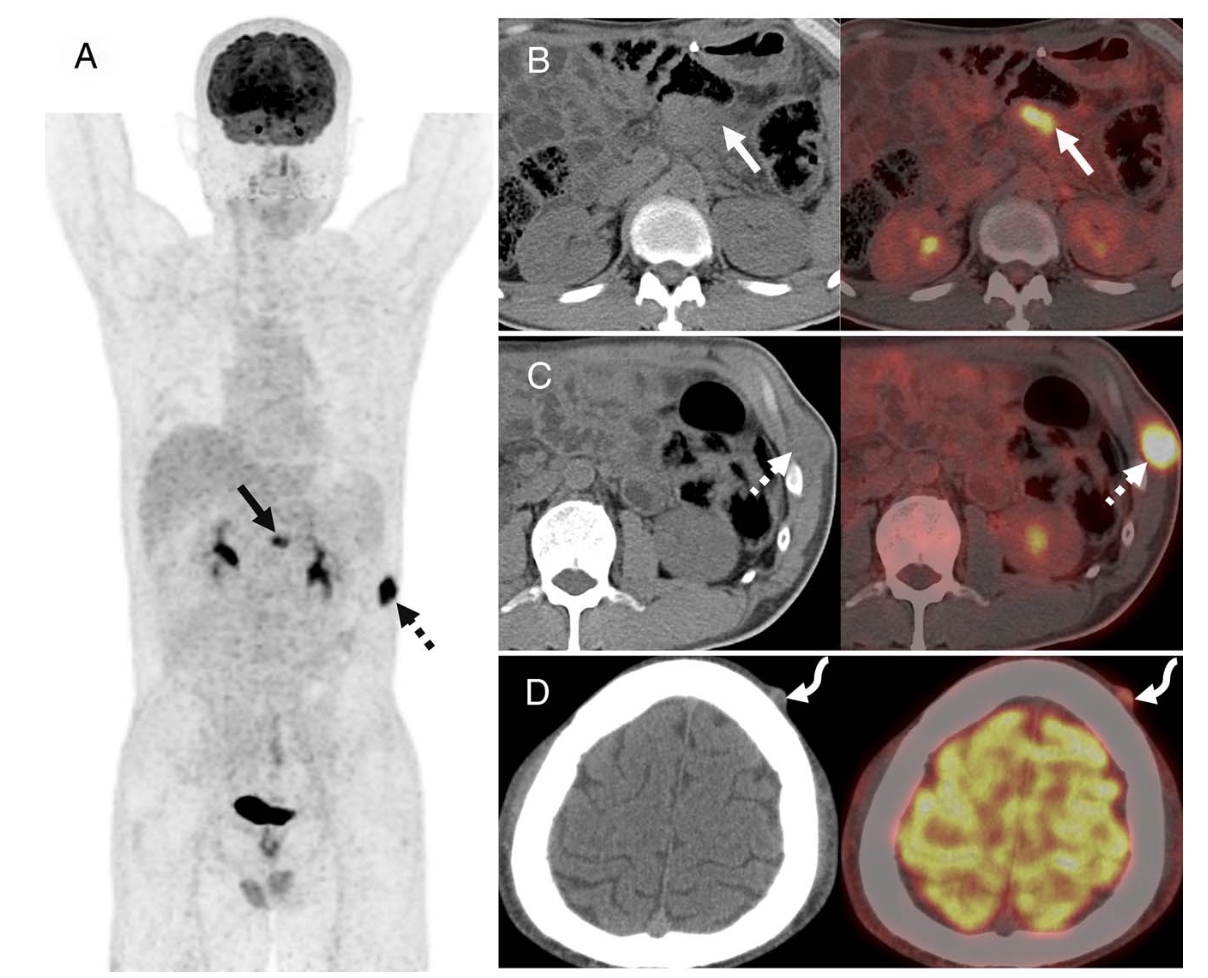
\includegraphics[width=0.65\textwidth]{assets/Zhang1.png}
	\caption{Rare cutaneous and muscle metastases detected using FDG-PET/CT, illustrating its capability for identifying uncommon metastatic sites \cite{Zhang2023}.}
	\label{fig:Zhang1}
\end{figure}

%---

\begin{multicols}{2}

%Case 3 - Deng
\subsection{Tumor Localization and Metabolic Assessment}

\textbf{Metabolic Imaging in Practice:} As stated before the value of FDG-PET resides on the its ability to visualize regions of increased glucose metabolism, even in lesions not that well defined morphologically. A case application is the results of Deng et al. where PET/CT effectively detects hypermetabolic pancreatic tumors. But, new tracers like 68Ga-FAPI outperform FDG in identifying micrometastases, particularly in hypodense liver lesions \cite{Deng2021}. %differences on the isotope

This is the case of a 65-year-old man who presented with abdominal pain. Abdominal ultrasound revealed a mass in the head of the pancreas, and pancreatic cancer was suspected. Then, underwent 18F-FDG PET/CT for initial staging, but no significant FDG uptake was seen. Finally he agreed to be imaged using 68Ga-FAPI.

Figure~\ref{fig:DengMerged} illustrates the comparative uptake of 68Ga-FAPI and 18F-FDG in pancreatic cancer with liver metastases, in (a) We see the results of [18F]FDG radiotracer and (b) are images obtained using 68Ga-FAPI instead.

In figure~\ref{fig:DengMerged} (a) Mild FDG uptake was observed in the pancreatic mass (arrowhead) and bone destruction in the 10th rib on the right (hollow arrow. However, 68Ga-FAPI PET/CT revealed intense FAPI uptake in the pancreas and the 10th rib and multiple lesions in the liver (dashed and solid arrows). Axial views with each radiotracer are also shown. First, 18F-FDG PET/CT (a)[B,C,D] (upper: PET image; middle: CT scan; lower: PET/CT fused image) showed moderate uptake in the mass, which is the head of the pancreas (B, arrowhead) and mild uptake in the 10th rib (C, hollow arrow) with minimal bone destruction and small hypodense nodules (D, hyphenated arrows)

Second image with 68Ga-FAPI shows a maximal intensity projection image (A) and axial views (B–D, upper: PET image; middle: CT scan; lower: PET/CT fused image). It showed more intense uptake than 18F-FDG at the head of the pancreas (arrowheads, SUVmax = 18.6) and the 10th rib on the right side (hollow arrows, SUVmax = 4.9). In addition, on the axial views, diffused pancreatic uptake (arrows, SUVmax = 11.5) and multiple focal uptake of isodense or hypodense nodules in the liver (dashed arrows) were found. Finally, an endoscopic ultrasonography–guided biopsy confirmed carcinoma in the head of the pancreas with liver metastasis. 

\textbf{Quantitative Metrics in Action:} The metric of choice is the Standardized Uptake Value (SUV), it measures FDG uptake in a lesion relative to a reference. The lower the SUV the better as it correlates to malignancy. By knowing this parameter it is posiible to identify micrometastatic lesions, particularly in the liver. Deng et al. shows that 68Ga-FAPI has superior sensitivity highlighting it as a promising area for future research on radiotracers.\cite{Deng2021}

Section 4 demonstrated the utility that PET/CT provides to diagnosis, staging, and management of pancreatic cancer. These clinical cases are an example of the current technology and limitations that we have in terms of resolution and specificity, and accessibility. Addressing these limitations will lean this technology forward for better and precise treatment, innovations in radiotracer development and hybrid imaging modalities can certainly be the way forward.

\end{multicols}

% walk thru
\begin{figure}[ht]
	\centering
	\begin{subfigure}[b]{\textwidth}
		\centering
		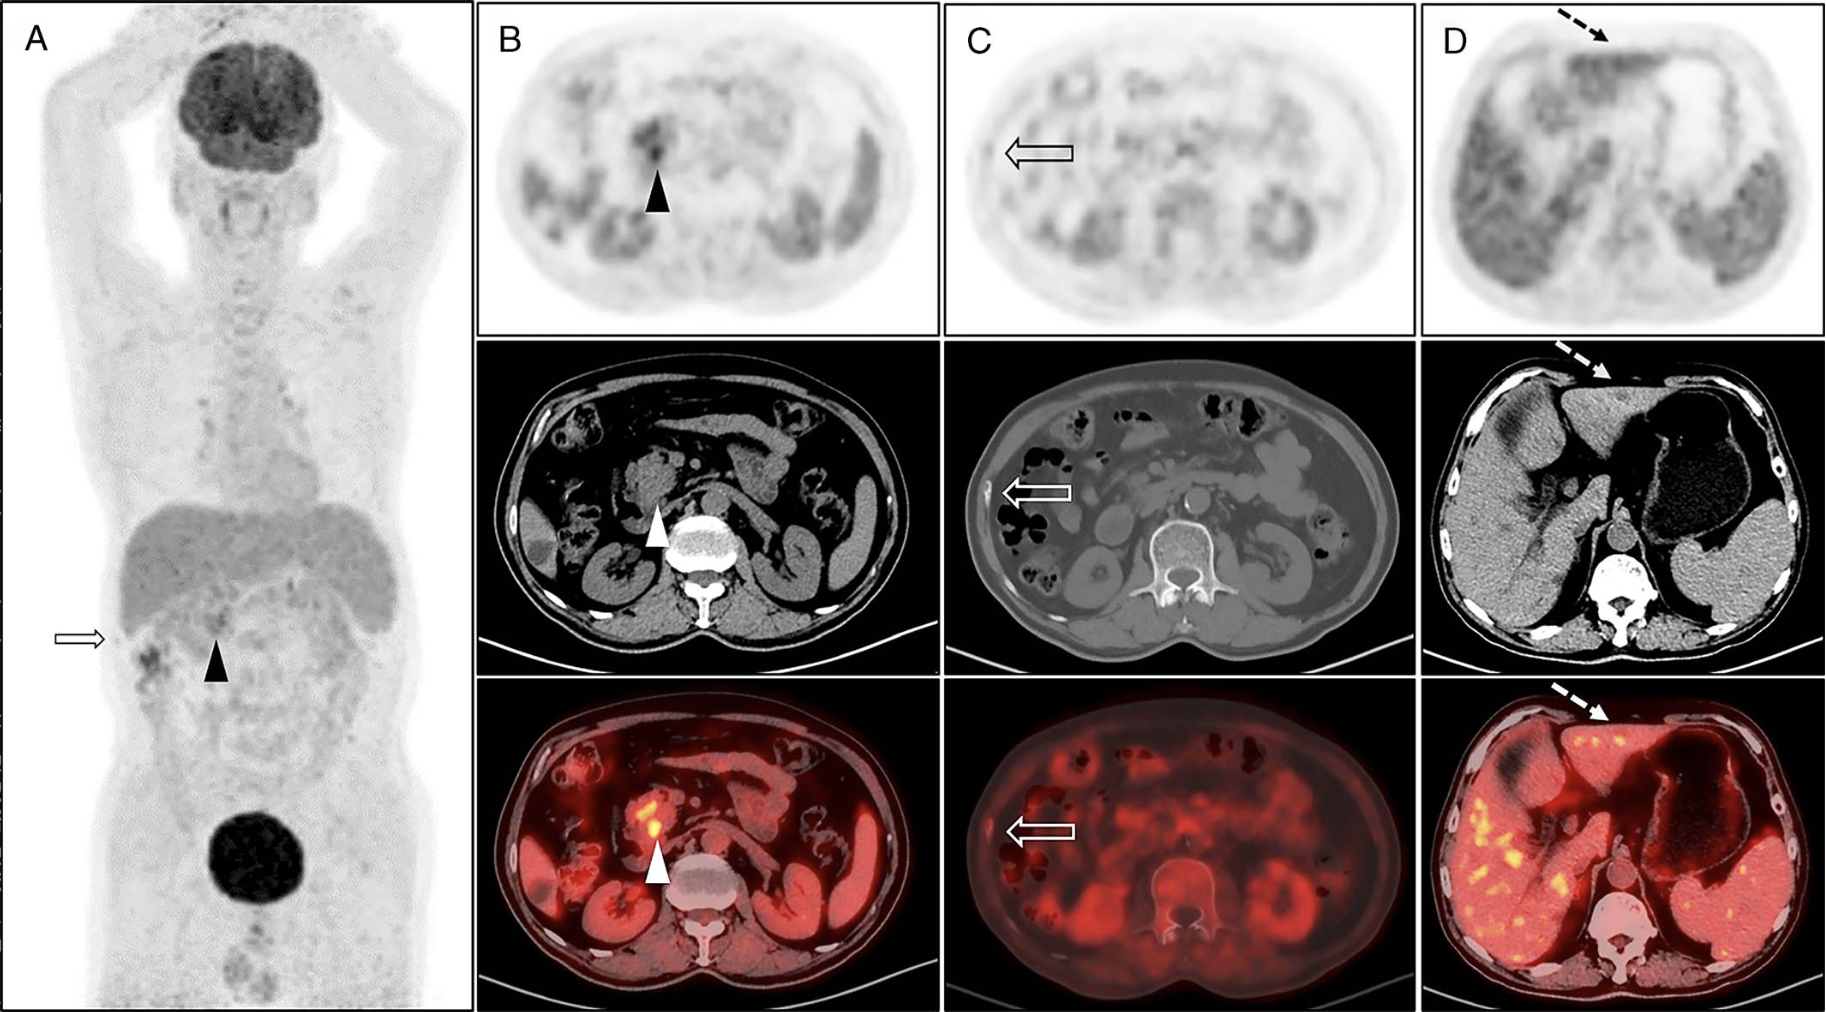
\includegraphics[width=\textwidth]{assets/Deng1.png}
		\caption{18F-FDG PET/CT showing pancreatic mass and liver hypodense lesions with minimal uptake, highlighting its sensitivity in tumor and liver staging \cite{Deng2021}.}
		\label{fig:Deng1}
	\end{subfigure}
	\vspace{1em} % Adjust vertical spacing
	\begin{subfigure}[b]{\textwidth}
		\centering
		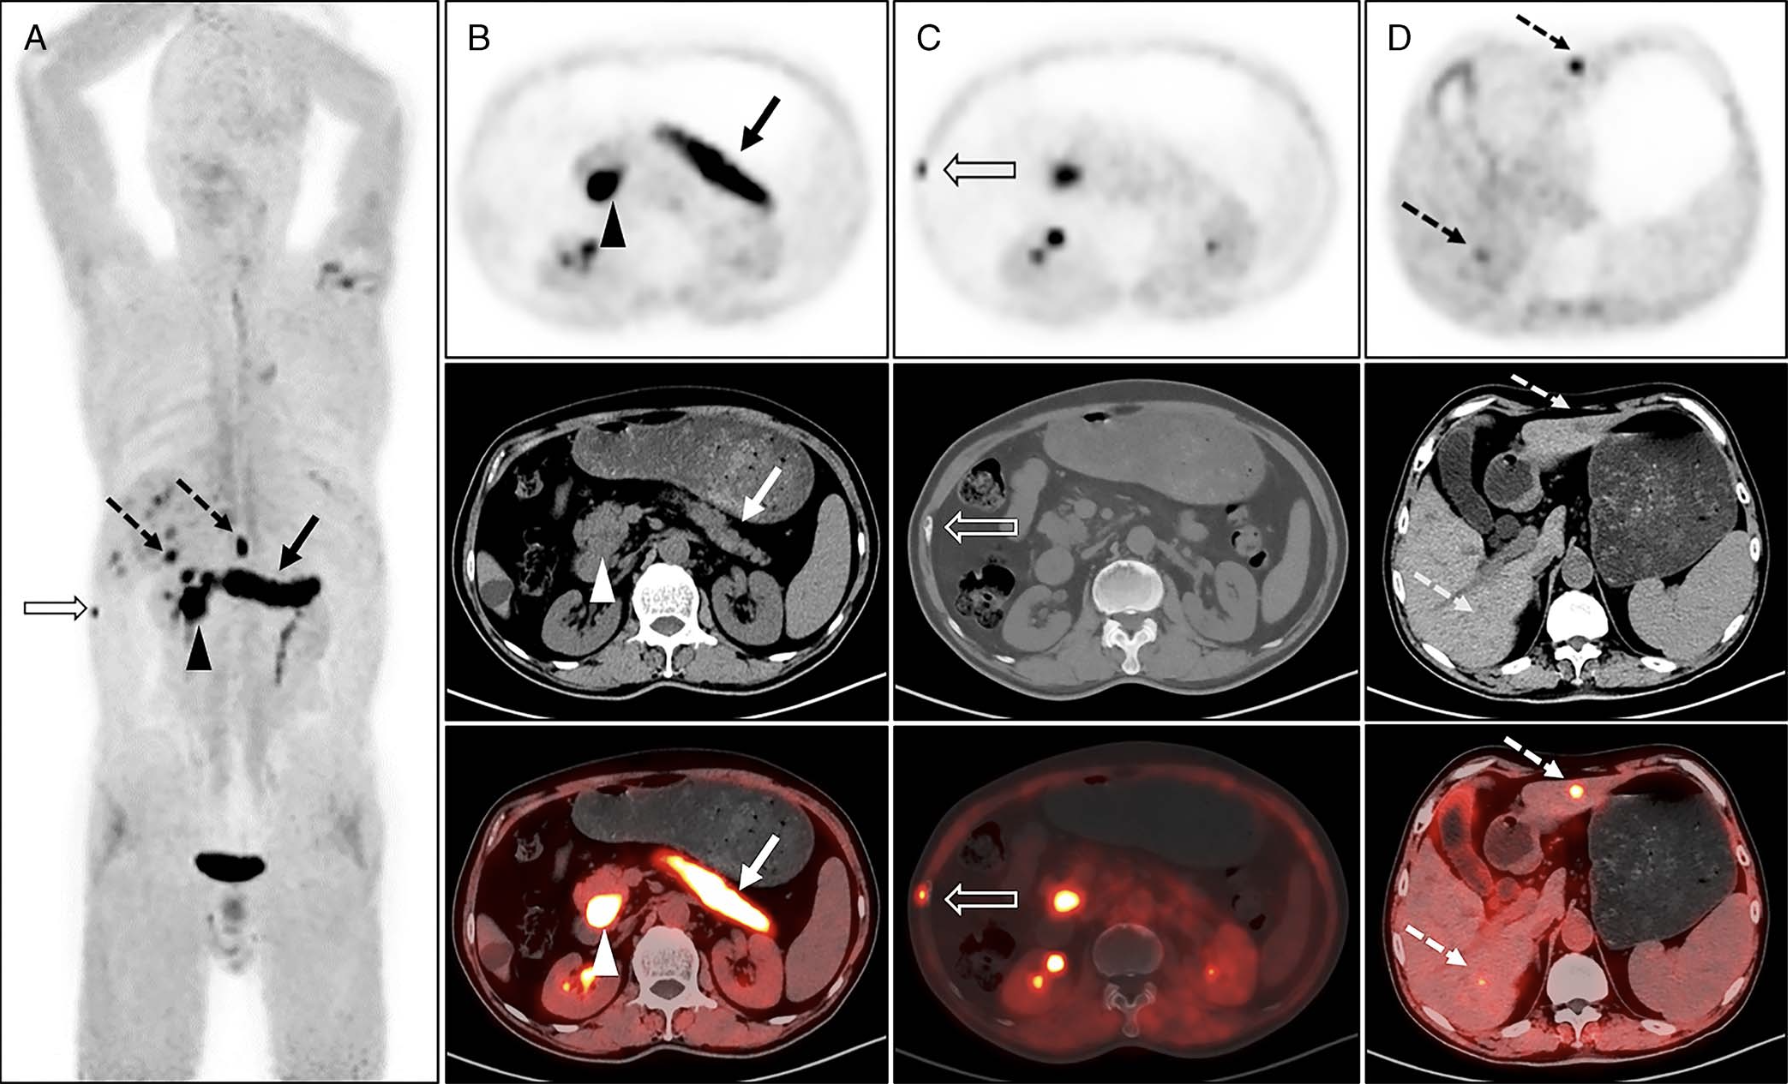
\includegraphics[width=\textwidth]{assets/Deng268GaComplete.png}
		\caption{Enhanced metabolic activity in pancreatic lesions with high resolution; 68Ga-FAPI tracer’s specificity in hypometabolic areas near the liver \cite{Deng2021}.}
		\label{fig:Deng268Ga}
	\end{subfigure}
	\caption{Comparison of FDG-PET/CT metabolic activity.}
	\label{fig:DengMerged}
\end{figure}

%---



\FloatBarrier % Prevents floats from going past this point